Kiến trúc vi dịch vụ chia dự án thành các thành phần nhỏ hơn được gọi là các dịch vụ.

Mỗi dịch vụ tập trung vào một khả năng kinh doanh cụ thể.

Các dịch vụ độc lập và giao tiếp với nhau thông qua hạ tầng mạng.

Trong thực tế, nhiều dự án thường chuyển đổi một cách dần dần từ kiến trúc nguyên khối sang kiến trúc vi dịch vụ.

\begin{figure}[H]

% Khi nào Vẽ lại chất lượng cao hơn

\centering

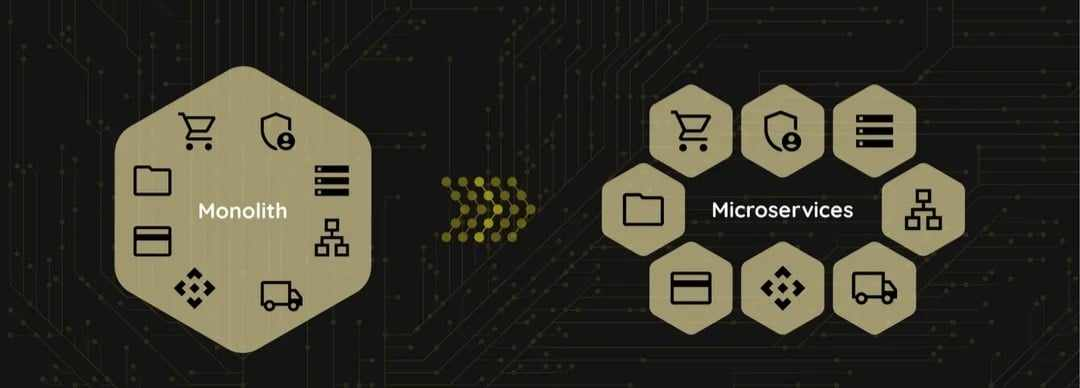
\includegraphics[scale = 0.4]{pictures/anh_khac_nhau_giua_kien_truc_nguyen_khoi_va_kien_truc_vi_dich_vu/main.jpg}

\caption{Ảnh khác nhau giữa kiến trúc nguyên khối và kiến trúc vi dịch vụ}

\end{figure}

